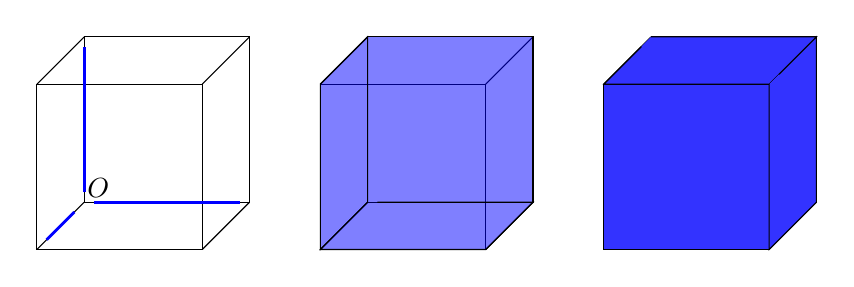
\begin{tikzpicture}[scale=0.6]
\tikzstyle{visited}=[line width=1pt,blue];

\draw  (-2.5,1.5) node (v2) {} rectangle (1,-2) node (v4) {};
\draw  (-1.5,2.5) node (v1) {} rectangle (2,-1) node (v3) {};
\draw (1,1.5) -- (2,2.5);
\draw (-1.5,-1) node (v7) {} -- (-2.5,-2) node (v9) {};
\draw (2,-1) node (v10) {} --  (1,-2);
\draw  (-1.5,2.5) node (v8) {} --  (-2.5,1.5) ;

\draw (7,1.5) -- (8,2.5);
\draw (4.5,-1) node (v11) {} -- (3.5,-2) node (v12) {};
\draw (8,-1) --  (7,-2);
\draw  (4.5,2.5) node (v6) {} --  (3.5,1.5) node (v5) {} ;
\draw  (v5) rectangle (7,-2) node (v15) {};
\draw [fill=blue,fill opacity=0.5] (v6) rectangle (8,-1) node (v16) {};
\draw [fill=blue,fill opacity=0.5] (4.5,2.5) --  (4.5,-1) node (v13) {} -- (3.5,-2) node (v14) {} -- (3.5,1.5) -- cycle;
\draw [fill=blue,fill opacity=0.5] (4.5,-1) -- (3.5,-2) -- (7,-2) -- (8,-1) -- (v13);

\draw (13,1.5) -- (14,2.5) node (v17) {};
\draw (10.5,-1) -- (9.5,-2);
\draw (14,-1) --  (13,-2);
\draw  (10.5,2.5) node (v6) {} --  (9.5,1.5) node (v5) {} ;
\draw  (v6) rectangle (14,-1) node (v20) {};
\draw [fill=blue!80]  (v5) rectangle (13,-2) node (v19) {};

\draw [visited] (v7) edge (v8);
\draw [visited] (v7) edge (v9);
\draw [visited] (v7) edge (v10);

\draw[fill=blue!80] (v6) -- (9.5,1.5) -- (13,1.5) node (v18) {} -- (14,2.5) node (v21) {} -- (10.5,2.5);

\draw[fill=blue!80] (13,1.5) -- (13,-2) --  (14,-1)  --(14,2.5)-- (v18);
\node at (-1.2,-0.7) {$O$};
\end{tikzpicture}